\documentclass[10pt,twocolumn,letterpaper]{article}
% ICCV Rules:
% 8 page limit (6 free + 2 paid)
% 10MB pdf file size limit
% 30MB supplementary materials file size limit (PDF or ZIP)

\usepackage{cvpr}
\usepackage[pagebackref=true,breaklinks=true,letterpaper=true,colorlinks,bookmarks=false]{hyperref}
\usepackage{times}
\usepackage{epsfig}
\usepackage{graphicx}
\usepackage{amsmath}
\usepackage{amssymb}
\usepackage{amsfonts}
\usepackage{algorithm}
\usepackage{algorithmic}
\usepackage{subfigure}

% Needed for getting formulas in dia diagrams.
\usepackage{pstricks}
\usepackage{tikz}

\usepackage{mydefs}

% \cvprfinalcopy % *** Uncomment this line for the final submission

\def\cvprPaperID{184} % *** Enter the CVPR Paper ID here
\def\httilde{\mbox{\tt\raisebox{-.5ex}{\symbol{126}}}}

% Pages are numbered in submission mode, and unnumbered in camera-ready
\ifcvprfinal\pagestyle{empty}\fi
\begin{document}

%\title{Accelerating $\ell_1$-Minimization Using Many-Core CPUs/GPUs \\ and Application to Face Recognition
%\title{Efficient Parallelization of Sparse Representation for Face Recognition}
%\thanks{Corresponding author: . This work was partially supported by ARO MURI W911NF-06-1-0076.}}
%\title{Many-Core Parallelization of $\ell_1$-Minimization for Face Recognition
\title{Parallelization of Fast $\ell_1$-Minimization for Face Recognition}

\author{First Author\\
Institution1\\
Institution1 address\\
{\tt\small firstauthor@i1.org}
% For a paper whose authors are all at the same institution,
% omit the following lines up until the closing ``}''.
% Additional authors and addresses can be added with ``\and'',
% just like the second author.
% To save space, use either the email address or home page, not both
\and
Second Author\\
Institution2\\
First line of institution2 address\\
{\small\url{http://www.author.org/~second}}
}

\maketitle

\begin{abstract} 
Recently a family of promising face recognition algorithms that are based on sparse representation and $\ell_1$ minimization have been been developed.  These algorithms have not yet seen commercial application, largely due to their greater computational requirements compared to more traditional algorithms.  This paper studies techniques for leveraging the massive parallelism available in GPU and multi-core CPU hardware to accelerate augmented Lagrangian method (ALM) based $\ell_1$ minimization solvers.  The proposed implementations are significantly faster than than previously published implementations.  Despite the low arithmetic intensity of ALM solvers, the GPU can still outperform the CPU by a wide margin for large problem sizes, and when solving many small problems simultaneously.  The proposed CPU implementation remains faster for solving a single moderately sized problem.  
\end{abstract}

\section{Introduction} 
$\ell_1$ minimization ($\ell_1$-min) has received much attention in recent
years due to important applications in compressive sensing
\cite{BrucksteinA2007} and sparse representation \cite{WrightJ2010-PIEEE}.  
$\ell_1$-min refers to finding the minimum $\ell_1$-norm solution to an
underdetermined linear system $\bb=A\xx$:
\begin{equation}
\min \|\xx\|_1\quad \mbox{ subj. to }\quad \bb = A\xx.
\label{eq:l1min}
\end{equation}
It is now well established that, under certain conditions
\cite{CandesE2005-IT_1,DonohoD2004}, the minimum $\ell_1$-norm solution is also
the \emph{sparsest} solution to the system \eqref{eq:l1min}.

Among its many applications, $\ell_1$-min has been recently used to reformulate
image-based face recognition as a sparse representation problem
\cite{WrightJ2009-PAMI}.  If we stack the training images of $K$ subject
classes $(A_1\in\Re^{d\times n_1}, \cdots, A_K\in\Re^{d\times n_K})$ into the
columns of a matrix $A = [A_1, \cdots, A_K]\in\Re^{d\times n}$, given a new
query image in the same vector form $\bb\in\Re^d$, \emph{sparsity-based
classification} (SBC) solves the following minimization problem:
\begin{equation}
\min_{\xx, \ee} \| \xx \|_1 + \|\ee\|_1 \quad \subj \quad \bb = A \xx + \ee.
\label{eq:l1min_denoise}
\end{equation}
If the sparsest solutions for $\x$ and $\e$ are recovered, $\ee$ provides a
means to compensate for pixels that are corrupted due to occlusion of some part of the query
image, and the dominant nonzero coefficients of $\xx$ reveal the membership of
$\bb$ based on the training image labels associated with $A$.  Since $A$ ideally
contains many images per user taken under different illuminations, 
$A\x$ also acts as a linear illumination model for the test image $\bb$.

In this paper, we study parallelization of $\ell$-min on many-core CPU and GPU
architectures. Although $\ell_1$-min \eqref{eq:l1min} is a convex
program, conventional algorithms such as interior-point methods
\cite{ChenS2001-SIAM,TibshiraniR1996} are known to suffer from poor scalability
for large-scale applications such as face recognition. Recently, a number of
accelerated algorithms have been proposed that explicitly take advantage of
the special structure of $\ell_1$-min problems
\cite{LorisI2009,YangA2010-ICIP}. We investigate parallelization of a
state-of-the-art $\ell_1$-min solution based on the classical framework of
\emph{augmented Lagrangian methods} (ALM) \cite{BertsekasD2003,YangA2010-ICIP}.

While solving \eqref{eq:l1min_denoise} can achieve exceptional
recognition accuracy on public databases, its success also relies on the assumption
that the query image is well aligned with the training images. In
\cite{WagnerA2009-CVPR}, the framework of SBC was extended to iteratively align
a query image to each subject class individually. The face alignment algorithm solves
the following minimization problem:
\begin{equation}
\hat{\tau}_i = \arg\min_{\xx, \ee, \tau_i} \|\ee\|_1\quad \mbox{subj. to}\quad \tilde\bb\circ\tau_i = A_i\xx + \ee,
\label{eq:l1min_alignment}
\end{equation}
where $\tau_i\in T$ is in a finite-dimensional group $T$ of transformations
(e.g., affine or homography) acting on the image domain.  The sequence
$\tau_i$ converges to a transformation that aligns the test image $\tilde\bb$
with the training images from the $i$-th class $A_i$. In other words, the algorithm 
extends Lucas-Kanade iterative alignment \cite{LucasB1981} to use the
$\ell_1$-norm as a robust error function, while simultaneously estimating
the coefficients of the linear illumination model $A\x$.  

Numerically, the original solution \cite{WagnerA2009-CVPR} was implemented based 
on standard interior-point methods, and its speed has been since improved by ALM in a more recent paper
\cite{WagnerA2011-PAMI}. However, due the high per-class cost
of the alignment step, the recognition system still fails to achieve real-time recognition against datasets of hundreds or thousands of users.
In this paper, in addition to accelerating the generic
$\ell_1$-min objectives \eqref{eq:l1min} and \eqref{eq:l1min_denoise}, we 
also discuss how to properly accelerate the iterative face alignment step
\eqref{eq:l1min_alignment} on multi-core CPUs and GPUs.

In this discussion we will clearly distinguish between algorithm {\em parallelism},
which is a property of an algorithm, and hardware {\em concurrency}, which is a
property of a hardware architecture. Parallelism in an algorithm provides the
opportunity to perform computations concurrently on hardware.  Algorithms often
exhibit multiple levels of parallelism, and hardware often provides multiple
levels of concurrency.  In these terms, the primary contribution of this paper
will be to determine the optimal mappings between the parallelism available in
$\ell_1$-min and the concurrency available in multi-core CPU and GPU
architectures.

Finally, we present extensive benchmark to compare the performance of the
generic ALM $\ell_1$-min algorithm and the corresponding face recognition
routines on massively parallel CPUs and GPUs.  To this end, a face
recognition system for security and access control applications has been implemented, 
and is diagrammed in Figure \ref{fig:pipeline}. This pipeline follows the work of \cite{WagnerA2011-PAMI}, but
the fast implementations presented in this paper are novel.
Since the parallelization of any algorithm
is highly dependent on the target hardware, we will give a brief overview of
the architecture of our test system in detail in Section
\ref{sec:concurrency}.
Finally, note that 
while this paper focuses on the parallelism available in a single (shared memory) machine,
applications targeting thousands of users or more, will likely require computation be
distributed over a cluster or network of computers, and this is not addressed here.
The source code of our implementations, which target Nvidia's CUDA GPU architecture,
as well as the x86-64 architecture, will be made available for peer evaluation.
\begin{figure}
\centering
{\tiny % Graphic for TeX using PGF
% Title: pipeline_simplified.dia
% Creator: Dia v0.97-pre3
% CreationDate: Mon Feb 14 03:20:49 2011
% For: awagner
% \usepackage{tikz}
% The following commands are not supported in PSTricks at present
% We define them conditionally, so when they are implemented,
% this pgf file will use them.
\ifx\du\undefined
  \newlength{\du}
\fi
\setlength{\du}{15\unitlength}
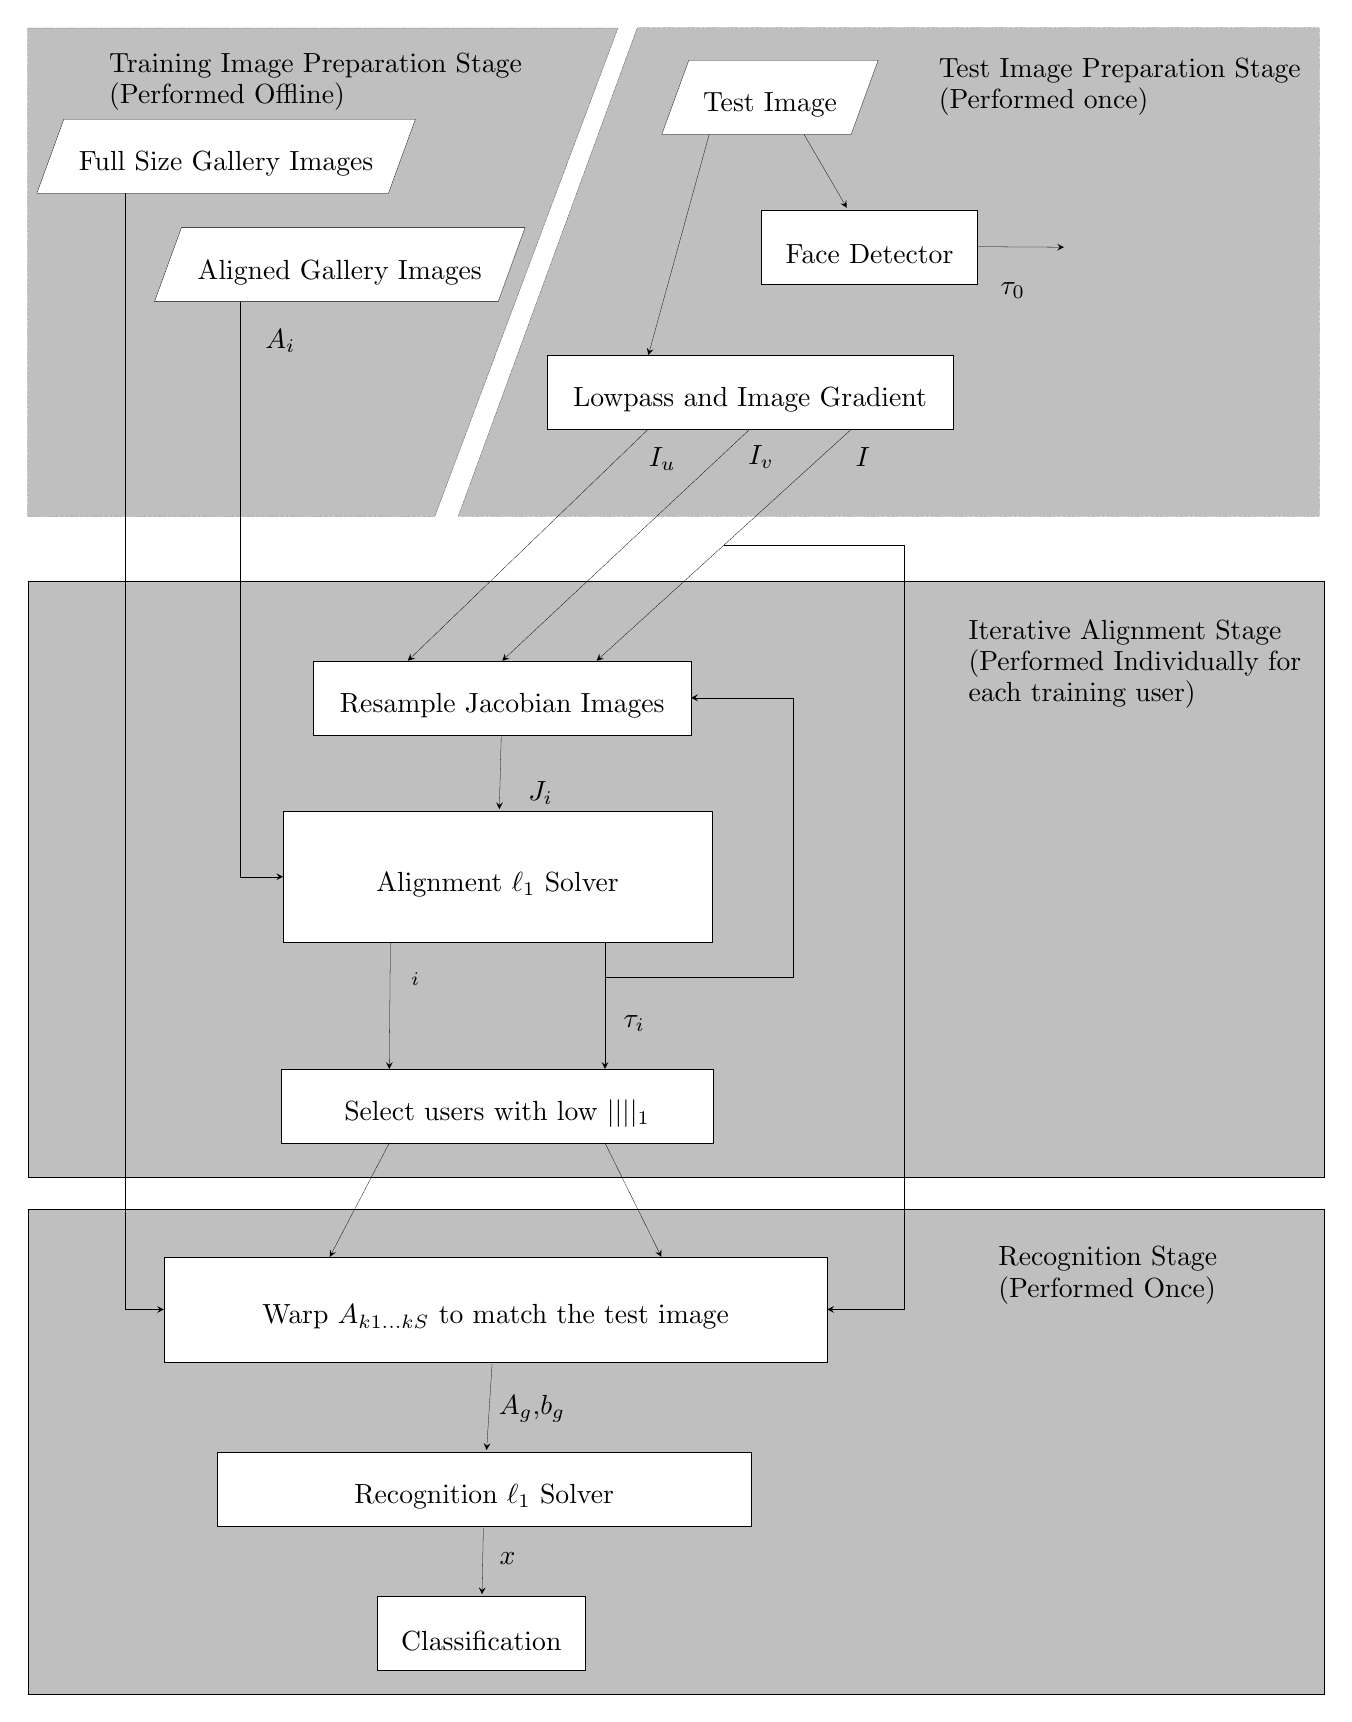
\begin{tikzpicture}
\pgftransformxscale{0.494667}
\pgftransformyscale{-0.494667}
\definecolor{dialinecolor}{rgb}{0.000000, 0.000000, 0.000000}
\pgfsetstrokecolor{dialinecolor}
\definecolor{dialinecolor}{rgb}{1.000000, 1.000000, 1.000000}
\pgfsetfillcolor{dialinecolor}
% setfont left to latex
\definecolor{dialinecolor}{rgb}{0.000000, 0.000000, 0.000000}
\pgfsetstrokecolor{dialinecolor}
\node[anchor=west] at (24.925000\du,42.952500\du){};
% setfont left to latex
\definecolor{dialinecolor}{rgb}{0.000000, 0.000000, 0.000000}
\pgfsetstrokecolor{dialinecolor}
\node[anchor=west] at (24.925000\du,42.952500\du){};
% setfont left to latex
\definecolor{dialinecolor}{rgb}{0.000000, 0.000000, 0.000000}
\pgfsetstrokecolor{dialinecolor}
\node[anchor=west] at (24.925000\du,42.952500\du){};
\definecolor{dialinecolor}{rgb}{0.749020, 0.749020, 0.749020}
\pgfsetfillcolor{dialinecolor}
\fill (6.494040\du,27.943300\du)--(6.494040\du,43.255071\du)--(39.770015\du,43.255071\du)--(39.770015\du,27.943300\du)--cycle;
\pgfsetlinewidth{0.100000\du}
\pgfsetdash{{\pgflinewidth}{0.200000\du}}{0cm}
\pgfsetdash{{\pgflinewidth}{0.200000\du}}{0cm}
\pgfsetmiterjoin
\definecolor{dialinecolor}{rgb}{0.000000, 0.000000, 0.000000}
\pgfsetstrokecolor{dialinecolor}
\draw (6.494040\du,27.943300\du)--(6.494040\du,43.255071\du)--(39.770015\du,43.255071\du)--(39.770015\du,27.943300\du)--cycle;
% setfont left to latex
\definecolor{dialinecolor}{rgb}{0.000000, 0.000000, 0.000000}
\pgfsetstrokecolor{dialinecolor}
\node at (23.132027\du,35.794186\du){};
\definecolor{dialinecolor}{rgb}{0.749020, 0.749020, 0.749020}
\pgfsetfillcolor{dialinecolor}
\fill (6.494040\du,44.061200\du)--(6.494040\du,56.519596\du)--(39.770015\du,56.519596\du)--(39.770015\du,44.061200\du)--cycle;
\pgfsetlinewidth{0.100000\du}
\pgfsetdash{{\pgflinewidth}{0.200000\du}}{0cm}
\pgfsetdash{{\pgflinewidth}{0.200000\du}}{0cm}
\pgfsetmiterjoin
\definecolor{dialinecolor}{rgb}{0.000000, 0.000000, 0.000000}
\pgfsetstrokecolor{dialinecolor}
\draw (6.494040\du,44.061200\du)--(6.494040\du,56.519596\du)--(39.770015\du,56.519596\du)--(39.770015\du,44.061200\du)--cycle;
% setfont left to latex
\definecolor{dialinecolor}{rgb}{0.000000, 0.000000, 0.000000}
\pgfsetstrokecolor{dialinecolor}
\node at (23.132027\du,50.485398\du){};
% setfont left to latex
\definecolor{dialinecolor}{rgb}{0.000000, 0.000000, 0.000000}
\pgfsetstrokecolor{dialinecolor}
\node[anchor=west] at (23.132000\du,35.599200\du){};
% setfont left to latex
\definecolor{dialinecolor}{rgb}{0.000000, 0.000000, 0.000000}
\pgfsetstrokecolor{dialinecolor}
\node[anchor=west] at (23.132000\du,35.599200\du){};
% setfont left to latex
\definecolor{dialinecolor}{rgb}{0.000000, 0.000000, 0.000000}
\pgfsetstrokecolor{dialinecolor}
\node[anchor=west] at (30.406100\du,29.259100\du){Iterative Alignment Stage};
% setfont left to latex
\definecolor{dialinecolor}{rgb}{0.000000, 0.000000, 0.000000}
\pgfsetstrokecolor{dialinecolor}
\node[anchor=west] at (30.406100\du,30.059100\du){(Performed Individually for};
% setfont left to latex
\definecolor{dialinecolor}{rgb}{0.000000, 0.000000, 0.000000}
\pgfsetstrokecolor{dialinecolor}
\node[anchor=west] at (30.406100\du,30.859100\du){each training user)};
% setfont left to latex
\definecolor{dialinecolor}{rgb}{0.000000, 0.000000, 0.000000}
\pgfsetstrokecolor{dialinecolor}
\node[anchor=west] at (31.173700\du,45.350700\du){Recognition Stage};
% setfont left to latex
\definecolor{dialinecolor}{rgb}{0.000000, 0.000000, 0.000000}
\pgfsetstrokecolor{dialinecolor}
\node[anchor=west] at (31.173700\du,46.150700\du){(Performed Once)};
\pgfsetlinewidth{0.100000\du}
\pgfsetdash{{\pgflinewidth}{0.200000\du}}{0cm}
\pgfsetdash{{\pgflinewidth}{0.200000\du}}{0cm}
\pgfsetmiterjoin
\pgfsetbuttcap
\definecolor{dialinecolor}{rgb}{0.749020, 0.749020, 0.749020}
\pgfsetfillcolor{dialinecolor}
\fill (6.494040\du,13.746400\du)--(21.645100\du,13.746400\du)--(16.943000\du,26.285100\du)--(6.494040\du,26.285100\du)--cycle;
\definecolor{dialinecolor}{rgb}{0.000000, 0.000000, 0.000000}
\pgfsetstrokecolor{dialinecolor}
\draw (6.494040\du,13.746400\du)--(21.645100\du,13.746400\du)--(16.943000\du,26.285100\du)--(6.494040\du,26.285100\du)--cycle;
% setfont left to latex
\definecolor{dialinecolor}{rgb}{0.000000, 0.000000, 0.000000}
\pgfsetstrokecolor{dialinecolor}
\node[anchor=west] at (8.342710\du,14.710900\du){Training Image Preparation Stage};
% setfont left to latex
\definecolor{dialinecolor}{rgb}{0.000000, 0.000000, 0.000000}
\pgfsetstrokecolor{dialinecolor}
\node[anchor=west] at (8.342710\du,15.510900\du){(Performed Offline)};
\pgfsetlinewidth{0.100000\du}
\pgfsetdash{{\pgflinewidth}{0.200000\du}}{0cm}
\pgfsetdash{{\pgflinewidth}{0.200000\du}}{0cm}
\pgfsetmiterjoin
\pgfsetbuttcap
\definecolor{dialinecolor}{rgb}{0.749020, 0.749020, 0.749020}
\pgfsetfillcolor{dialinecolor}
\fill (22.141100\du,13.740100\du)--(39.649500\du,13.740100\du)--(39.649500\du,26.278900\du)--(17.545800\du,26.278900\du)--cycle;
\definecolor{dialinecolor}{rgb}{0.000000, 0.000000, 0.000000}
\pgfsetstrokecolor{dialinecolor}
\draw (22.141100\du,13.740100\du)--(39.649500\du,13.740100\du)--(39.649500\du,26.278900\du)--(17.545800\du,26.278900\du)--cycle;
% setfont left to latex
\definecolor{dialinecolor}{rgb}{0.000000, 0.000000, 0.000000}
\pgfsetstrokecolor{dialinecolor}
\node[anchor=west] at (29.642500\du,14.831400\du){Test Image Preparation Stage};
% setfont left to latex
\definecolor{dialinecolor}{rgb}{0.000000, 0.000000, 0.000000}
\pgfsetstrokecolor{dialinecolor}
\node[anchor=west] at (29.642500\du,15.631400\du){(Performed once)};
\definecolor{dialinecolor}{rgb}{1.000000, 1.000000, 1.000000}
\pgfsetfillcolor{dialinecolor}
\fill (23.464443\du,14.572100\du)--(28.325620\du,14.572100\du)--(27.634076\du,16.472100\du)--(22.772900\du,16.472100\du)--cycle;
\pgfsetlinewidth{0.100000\du}
\pgfsetdash{}{0pt}
\pgfsetdash{}{0pt}
\pgfsetmiterjoin
\definecolor{dialinecolor}{rgb}{0.000000, 0.000000, 0.000000}
\pgfsetstrokecolor{dialinecolor}
\draw (23.464443\du,14.572100\du)--(28.325620\du,14.572100\du)--(27.634076\du,16.472100\du)--(22.772900\du,16.472100\du)--cycle;
% setfont left to latex
\definecolor{dialinecolor}{rgb}{0.000000, 0.000000, 0.000000}
\pgfsetstrokecolor{dialinecolor}
\node at (25.549260\du,15.717100\du){Test Image};
\definecolor{dialinecolor}{rgb}{1.000000, 1.000000, 1.000000}
\pgfsetfillcolor{dialinecolor}
\fill (13.826900\du,29.990700\du)--(13.826900\du,31.890700\du)--(23.521900\du,31.890700\du)--(23.521900\du,29.990700\du)--cycle;
\pgfsetlinewidth{0.100000\du}
\pgfsetdash{}{0pt}
\pgfsetdash{}{0pt}
\pgfsetmiterjoin
\definecolor{dialinecolor}{rgb}{0.000000, 0.000000, 0.000000}
\pgfsetstrokecolor{dialinecolor}
\draw (13.826900\du,29.990700\du)--(13.826900\du,31.890700\du)--(23.521900\du,31.890700\du)--(23.521900\du,29.990700\du)--cycle;
% setfont left to latex
\definecolor{dialinecolor}{rgb}{0.000000, 0.000000, 0.000000}
\pgfsetstrokecolor{dialinecolor}
\node at (18.674400\du,31.135700\du){Resample Jacobian Images};
\definecolor{dialinecolor}{rgb}{1.000000, 1.000000, 1.000000}
\pgfsetfillcolor{dialinecolor}
\fill (13.050000\du,33.850000\du)--(13.050000\du,37.221200\du)--(24.058800\du,37.221200\du)--(24.058800\du,33.850000\du)--cycle;
\pgfsetlinewidth{0.100000\du}
\pgfsetdash{}{0pt}
\pgfsetdash{}{0pt}
\pgfsetmiterjoin
\definecolor{dialinecolor}{rgb}{0.000000, 0.000000, 0.000000}
\pgfsetstrokecolor{dialinecolor}
\draw (13.050000\du,33.850000\du)--(13.050000\du,37.221200\du)--(24.058800\du,37.221200\du)--(24.058800\du,33.850000\du)--cycle;
% setfont left to latex
\definecolor{dialinecolor}{rgb}{0.000000, 0.000000, 0.000000}
\pgfsetstrokecolor{dialinecolor}
\node at (18.554400\du,35.730600\du){Alignment $\ell_1$ Solver};
\pgfsetlinewidth{0.100000\du}
\pgfsetdash{}{0pt}
\pgfsetdash{}{0pt}
\pgfsetbuttcap
{
\definecolor{dialinecolor}{rgb}{0.000000, 0.000000, 0.000000}
\pgfsetfillcolor{dialinecolor}
% was here!!!
\pgfsetarrowsend{stealth}
\definecolor{dialinecolor}{rgb}{0.000000, 0.000000, 0.000000}
\pgfsetstrokecolor{dialinecolor}
\draw (18.648326\du,31.939104\du)--(18.599693\du,33.801294\du);
}
% setfont left to latex
\definecolor{dialinecolor}{rgb}{0.000000, 0.000000, 0.000000}
\pgfsetstrokecolor{dialinecolor}
\node[anchor=west] at (11.250000\du,34.890000\du){};
\definecolor{dialinecolor}{rgb}{1.000000, 1.000000, 1.000000}
\pgfsetfillcolor{dialinecolor}
\fill (19.817600\du,22.143000\du)--(19.817600\du,24.043000\du)--(30.250100\du,24.043000\du)--(30.250100\du,22.143000\du)--cycle;
\pgfsetlinewidth{0.100000\du}
\pgfsetdash{}{0pt}
\pgfsetdash{}{0pt}
\pgfsetmiterjoin
\definecolor{dialinecolor}{rgb}{0.000000, 0.000000, 0.000000}
\pgfsetstrokecolor{dialinecolor}
\draw (19.817600\du,22.143000\du)--(19.817600\du,24.043000\du)--(30.250100\du,24.043000\du)--(30.250100\du,22.143000\du)--cycle;
% setfont left to latex
\definecolor{dialinecolor}{rgb}{0.000000, 0.000000, 0.000000}
\pgfsetstrokecolor{dialinecolor}
\node at (25.033850\du,23.288000\du){Lowpass and Image Gradient};
\definecolor{dialinecolor}{rgb}{1.000000, 1.000000, 1.000000}
\pgfsetfillcolor{dialinecolor}
\fill (25.332900\du,18.409900\du)--(25.332900\du,20.309900\du)--(30.875400\du,20.309900\du)--(30.875400\du,18.409900\du)--cycle;
\pgfsetlinewidth{0.100000\du}
\pgfsetdash{}{0pt}
\pgfsetdash{}{0pt}
\pgfsetmiterjoin
\definecolor{dialinecolor}{rgb}{0.000000, 0.000000, 0.000000}
\pgfsetstrokecolor{dialinecolor}
\draw (25.332900\du,18.409900\du)--(25.332900\du,20.309900\du)--(30.875400\du,20.309900\du)--(30.875400\du,18.409900\du)--cycle;
% setfont left to latex
\definecolor{dialinecolor}{rgb}{0.000000, 0.000000, 0.000000}
\pgfsetstrokecolor{dialinecolor}
\node at (28.104150\du,19.554900\du){Face Detector};
\definecolor{dialinecolor}{rgb}{1.000000, 1.000000, 1.000000}
\pgfsetfillcolor{dialinecolor}
\fill (9.987950\du,45.295200\du)--(9.987950\du,47.995200\du)--(27.017950\du,47.995200\du)--(27.017950\du,45.295200\du)--cycle;
\pgfsetlinewidth{0.100000\du}
\pgfsetdash{}{0pt}
\pgfsetdash{}{0pt}
\pgfsetmiterjoin
\definecolor{dialinecolor}{rgb}{0.000000, 0.000000, 0.000000}
\pgfsetstrokecolor{dialinecolor}
\draw (9.987950\du,45.295200\du)--(9.987950\du,47.995200\du)--(27.017950\du,47.995200\du)--(27.017950\du,45.295200\du)--cycle;
% setfont left to latex
\definecolor{dialinecolor}{rgb}{0.000000, 0.000000, 0.000000}
\pgfsetstrokecolor{dialinecolor}
\node at (18.502950\du,46.840200\du){Warp $A_{k1 \ldots kS}$ to match the test image};
\definecolor{dialinecolor}{rgb}{1.000000, 1.000000, 1.000000}
\pgfsetfillcolor{dialinecolor}
\fill (15.470400\du,54.006500\du)--(15.470400\du,55.906500\du)--(20.802900\du,55.906500\du)--(20.802900\du,54.006500\du)--cycle;
\pgfsetlinewidth{0.100000\du}
\pgfsetdash{}{0pt}
\pgfsetdash{}{0pt}
\pgfsetmiterjoin
\definecolor{dialinecolor}{rgb}{0.000000, 0.000000, 0.000000}
\pgfsetstrokecolor{dialinecolor}
\draw (15.470400\du,54.006500\du)--(15.470400\du,55.906500\du)--(20.802900\du,55.906500\du)--(20.802900\du,54.006500\du)--cycle;
% setfont left to latex
\definecolor{dialinecolor}{rgb}{0.000000, 0.000000, 0.000000}
\pgfsetstrokecolor{dialinecolor}
\node at (18.136650\du,55.151500\du){Classification};
% setfont left to latex
\definecolor{dialinecolor}{rgb}{0.000000, 0.000000, 0.000000}
\pgfsetstrokecolor{dialinecolor}
\node[anchor=west] at (28.104200\du,19.359900\du){};
\pgfsetlinewidth{0.100000\du}
\pgfsetdash{}{0pt}
\pgfsetdash{}{0pt}
\pgfsetbuttcap
{
\definecolor{dialinecolor}{rgb}{0.000000, 0.000000, 0.000000}
\pgfsetfillcolor{dialinecolor}
% was here!!!
\pgfsetarrowsend{stealth}
\definecolor{dialinecolor}{rgb}{0.000000, 0.000000, 0.000000}
\pgfsetstrokecolor{dialinecolor}
\draw (25.033800\du,24.043000\du)--(18.674400\du,29.990700\du);
}
\pgfsetlinewidth{0.100000\du}
\pgfsetdash{}{0pt}
\pgfsetdash{}{0pt}
\pgfsetbuttcap
{
\definecolor{dialinecolor}{rgb}{0.000000, 0.000000, 0.000000}
\pgfsetfillcolor{dialinecolor}
% was here!!!
\pgfsetarrowsend{stealth}
\definecolor{dialinecolor}{rgb}{0.000000, 0.000000, 0.000000}
\pgfsetstrokecolor{dialinecolor}
\draw (22.425700\du,24.043000\du)--(16.250600\du,29.990700\du);
}
\pgfsetlinewidth{0.100000\du}
\pgfsetdash{}{0pt}
\pgfsetdash{}{0pt}
\pgfsetbuttcap
{
\definecolor{dialinecolor}{rgb}{0.000000, 0.000000, 0.000000}
\pgfsetfillcolor{dialinecolor}
% was here!!!
\pgfsetarrowsend{stealth}
\definecolor{dialinecolor}{rgb}{0.000000, 0.000000, 0.000000}
\pgfsetstrokecolor{dialinecolor}
\draw (27.641900\du,24.043000\du)--(21.098100\du,29.990700\du);
}
% setfont left to latex
\definecolor{dialinecolor}{rgb}{0.000000, 0.000000, 0.000000}
\pgfsetstrokecolor{dialinecolor}
\node[anchor=west] at (27.506000\du,24.761200\du){$I$};
% setfont left to latex
\definecolor{dialinecolor}{rgb}{0.000000, 0.000000, 0.000000}
\pgfsetstrokecolor{dialinecolor}
\node[anchor=west] at (22.199300\du,24.802400\du){$I_u$};
\pgfsetlinewidth{0.100000\du}
\pgfsetdash{}{0pt}
\pgfsetdash{}{0pt}
\pgfsetbuttcap
{
\definecolor{dialinecolor}{rgb}{0.000000, 0.000000, 0.000000}
\pgfsetfillcolor{dialinecolor}
% was here!!!
\pgfsetarrowsend{stealth}
\definecolor{dialinecolor}{rgb}{0.000000, 0.000000, 0.000000}
\pgfsetstrokecolor{dialinecolor}
\draw (23.988200\du,16.472100\du)--(22.425700\du,22.143000\du);
}
\pgfsetlinewidth{0.100000\du}
\pgfsetdash{}{0pt}
\pgfsetdash{}{0pt}
\pgfsetbuttcap
{
\definecolor{dialinecolor}{rgb}{0.000000, 0.000000, 0.000000}
\pgfsetfillcolor{dialinecolor}
% was here!!!
\pgfsetarrowsend{stealth}
\definecolor{dialinecolor}{rgb}{0.000000, 0.000000, 0.000000}
\pgfsetstrokecolor{dialinecolor}
\draw (26.418800\du,16.472100\du)--(27.520491\du,18.359816\du);
}
% setfont left to latex
\definecolor{dialinecolor}{rgb}{0.000000, 0.000000, 0.000000}
\pgfsetstrokecolor{dialinecolor}
\node[anchor=west] at (28.248200\du,27.724100\du){};
% setfont left to latex
\definecolor{dialinecolor}{rgb}{0.000000, 0.000000, 0.000000}
\pgfsetstrokecolor{dialinecolor}
\node[anchor=west] at (31.230200\du,20.488200\du){$\tau_0$};
\definecolor{dialinecolor}{rgb}{1.000000, 1.000000, 1.000000}
\pgfsetfillcolor{dialinecolor}
\fill (7.418823\du,16.086600\du)--(16.445000\du,16.086600\du)--(15.753456\du,17.986600\du)--(6.727280\du,17.986600\du)--cycle;
\pgfsetlinewidth{0.100000\du}
\pgfsetdash{}{0pt}
\pgfsetdash{}{0pt}
\pgfsetmiterjoin
\definecolor{dialinecolor}{rgb}{0.000000, 0.000000, 0.000000}
\pgfsetstrokecolor{dialinecolor}
\draw (7.418823\du,16.086600\du)--(16.445000\du,16.086600\du)--(15.753456\du,17.986600\du)--(6.727280\du,17.986600\du)--cycle;
% setfont left to latex
\definecolor{dialinecolor}{rgb}{0.000000, 0.000000, 0.000000}
\pgfsetstrokecolor{dialinecolor}
\node at (11.586140\du,17.231600\du){Full Size Gallery Images};
\pgfsetlinewidth{0.100000\du}
\pgfsetdash{}{0pt}
\pgfsetdash{}{0pt}
\pgfsetmiterjoin
\pgfsetbuttcap
{
\definecolor{dialinecolor}{rgb}{0.000000, 0.000000, 0.000000}
\pgfsetfillcolor{dialinecolor}
% was here!!!
\pgfsetarrowsend{stealth}
{\pgfsetcornersarced{\pgfpoint{0.000000\du}{0.000000\du}}\definecolor{dialinecolor}{rgb}{0.000000, 0.000000, 0.000000}
\pgfsetstrokecolor{dialinecolor}
\draw (11.952169\du,20.770000\du)--(11.952169\du,35.535600\du)--(13.050000\du,35.535600\du);
}}
\pgfsetlinewidth{0.100000\du}
\pgfsetdash{}{0pt}
\pgfsetdash{}{0pt}
\pgfsetbuttcap
{
\definecolor{dialinecolor}{rgb}{0.000000, 0.000000, 0.000000}
\pgfsetfillcolor{dialinecolor}
% was here!!!
\pgfsetarrowsend{stealth}
\definecolor{dialinecolor}{rgb}{0.000000, 0.000000, 0.000000}
\pgfsetstrokecolor{dialinecolor}
\draw (30.875400\du,19.359900\du)--(33.098700\du,19.372700\du);
}
\definecolor{dialinecolor}{rgb}{1.000000, 1.000000, 1.000000}
\pgfsetfillcolor{dialinecolor}
\fill (11.356800\du,50.303600\du)--(11.356800\du,52.203600\du)--(25.061036\du,52.203600\du)--(25.061036\du,50.303600\du)--cycle;
\pgfsetlinewidth{0.100000\du}
\pgfsetdash{}{0pt}
\pgfsetdash{}{0pt}
\pgfsetmiterjoin
\definecolor{dialinecolor}{rgb}{0.000000, 0.000000, 0.000000}
\pgfsetstrokecolor{dialinecolor}
\draw (11.356800\du,50.303600\du)--(11.356800\du,52.203600\du)--(25.061036\du,52.203600\du)--(25.061036\du,50.303600\du)--cycle;
% setfont left to latex
\definecolor{dialinecolor}{rgb}{0.000000, 0.000000, 0.000000}
\pgfsetstrokecolor{dialinecolor}
\node at (18.208918\du,51.448600\du){Recognition $\ell_1$ Solver};
\pgfsetlinewidth{0.100000\du}
\pgfsetdash{}{0pt}
\pgfsetdash{}{0pt}
\pgfsetmiterjoin
\pgfsetbuttcap
{
\definecolor{dialinecolor}{rgb}{0.000000, 0.000000, 0.000000}
\pgfsetfillcolor{dialinecolor}
% was here!!!
\pgfsetarrowsend{stealth}
{\pgfsetcornersarced{\pgfpoint{0.000000\du}{0.000000\du}}\definecolor{dialinecolor}{rgb}{0.000000, 0.000000, 0.000000}
\pgfsetstrokecolor{dialinecolor}
\draw (21.306600\du,37.221200\du)--(21.306600\du,38.050000\du)--(21.312500\du,38.050000\du)--(21.312500\du,40.470000\du);
}}
\pgfsetlinewidth{0.100000\du}
\pgfsetdash{}{0pt}
\pgfsetdash{}{0pt}
\pgfsetbuttcap
{
\definecolor{dialinecolor}{rgb}{0.000000, 0.000000, 0.000000}
\pgfsetfillcolor{dialinecolor}
% was here!!!
\pgfsetarrowsend{stealth}
\definecolor{dialinecolor}{rgb}{0.000000, 0.000000, 0.000000}
\pgfsetstrokecolor{dialinecolor}
\draw (15.802200\du,37.221200\du)--(15.775000\du,40.470000\du);
}
% setfont left to latex
\definecolor{dialinecolor}{rgb}{0.000000, 0.000000, 0.000000}
\pgfsetstrokecolor{dialinecolor}
\node[anchor=west] at (16.096600\du,38.150600\du){$\e_i$};
\pgfsetlinewidth{0.100000\du}
\pgfsetdash{}{0pt}
\pgfsetdash{}{0pt}
\pgfsetbuttcap
{
\definecolor{dialinecolor}{rgb}{0.000000, 0.000000, 0.000000}
\pgfsetfillcolor{dialinecolor}
% was here!!!
\pgfsetarrowsend{stealth}
\definecolor{dialinecolor}{rgb}{0.000000, 0.000000, 0.000000}
\pgfsetstrokecolor{dialinecolor}
\draw (18.189395\du,52.253907\du)--(18.156173\du,53.956193\du);
}
\pgfsetlinewidth{0.100000\du}
\pgfsetdash{}{0pt}
\pgfsetdash{}{0pt}
\pgfsetmiterjoin
\pgfsetbuttcap
{
\definecolor{dialinecolor}{rgb}{0.000000, 0.000000, 0.000000}
\pgfsetfillcolor{dialinecolor}
% was here!!!
\pgfsetarrowsend{stealth}
{\pgfsetcornersarced{\pgfpoint{0.000000\du}{0.000000\du}}\definecolor{dialinecolor}{rgb}{0.000000, 0.000000, 0.000000}
\pgfsetstrokecolor{dialinecolor}
\draw (24.370000\du,27.016800\du)--(28.999500\du,27.016800\du)--(28.999500\du,46.645200\du)--(27.018000\du,46.645200\du);
}}
\pgfsetlinewidth{0.100000\du}
\pgfsetdash{}{0pt}
\pgfsetdash{}{0pt}
\pgfsetbuttcap
{
\definecolor{dialinecolor}{rgb}{0.000000, 0.000000, 0.000000}
\pgfsetfillcolor{dialinecolor}
% was here!!!
\pgfsetarrowsend{stealth}
\definecolor{dialinecolor}{rgb}{0.000000, 0.000000, 0.000000}
\pgfsetstrokecolor{dialinecolor}
\draw (18.413613\du,48.045384\du)--(18.272699\du,50.253951\du);
}
% setfont left to latex
\definecolor{dialinecolor}{rgb}{0.000000, 0.000000, 0.000000}
\pgfsetstrokecolor{dialinecolor}
\node[anchor=west] at (18.367000\du,53.041300\du){$x$};
% setfont left to latex
\definecolor{dialinecolor}{rgb}{0.000000, 0.000000, 0.000000}
\pgfsetstrokecolor{dialinecolor}
\node[anchor=west] at (18.349600\du,49.203000\du){$A_g$,$b_g$};
% setfont left to latex
\definecolor{dialinecolor}{rgb}{0.000000, 0.000000, 0.000000}
\pgfsetstrokecolor{dialinecolor}
\node[anchor=west] at (24.755000\du,24.750000\du){$I_v$};
% setfont left to latex
\definecolor{dialinecolor}{rgb}{0.000000, 0.000000, 0.000000}
\pgfsetstrokecolor{dialinecolor}
\node[anchor=west] at (12.355000\du,21.787500\du){$A_i$};
% setfont left to latex
\definecolor{dialinecolor}{rgb}{0.000000, 0.000000, 0.000000}
\pgfsetstrokecolor{dialinecolor}
\node[anchor=west] at (19.105000\du,33.387500\du){$J_i$};
\definecolor{dialinecolor}{rgb}{1.000000, 1.000000, 1.000000}
\pgfsetfillcolor{dialinecolor}
\fill (10.437793\du,18.870000\du)--(19.261470\du,18.870000\du)--(18.569926\du,20.770000\du)--(9.746250\du,20.770000\du)--cycle;
\pgfsetlinewidth{0.100000\du}
\pgfsetdash{}{0pt}
\pgfsetdash{}{0pt}
\pgfsetmiterjoin
\definecolor{dialinecolor}{rgb}{0.000000, 0.000000, 0.000000}
\pgfsetstrokecolor{dialinecolor}
\draw (10.437793\du,18.870000\du)--(19.261470\du,18.870000\du)--(18.569926\du,20.770000\du)--(9.746250\du,20.770000\du)--cycle;
% setfont left to latex
\definecolor{dialinecolor}{rgb}{0.000000, 0.000000, 0.000000}
\pgfsetstrokecolor{dialinecolor}
\node at (14.503860\du,20.015000\du){Aligned Gallery Images};
\pgfsetlinewidth{0.100000\du}
\pgfsetdash{}{0pt}
\pgfsetdash{}{0pt}
\pgfsetmiterjoin
\pgfsetbuttcap
{
\definecolor{dialinecolor}{rgb}{0.000000, 0.000000, 0.000000}
\pgfsetfillcolor{dialinecolor}
% was here!!!
\pgfsetarrowsend{stealth}
{\pgfsetcornersarced{\pgfpoint{0.000000\du}{0.000000\du}}\definecolor{dialinecolor}{rgb}{0.000000, 0.000000, 0.000000}
\pgfsetstrokecolor{dialinecolor}
\draw (8.983824\du,17.986600\du)--(8.983824\du,46.645200\du)--(9.987950\du,46.645200\du);
}}
\pgfsetlinewidth{0.100000\du}
\pgfsetdash{}{0pt}
\pgfsetdash{}{0pt}
\pgfsetmiterjoin
\pgfsetbuttcap
{
\definecolor{dialinecolor}{rgb}{0.000000, 0.000000, 0.000000}
\pgfsetfillcolor{dialinecolor}
% was here!!!
\pgfsetarrowsend{stealth}
{\pgfsetcornersarced{\pgfpoint{0.000000\du}{0.000000\du}}\definecolor{dialinecolor}{rgb}{0.000000, 0.000000, 0.000000}
\pgfsetstrokecolor{dialinecolor}
\draw (21.300000\du,38.100000\du)--(26.150000\du,38.100000\du)--(26.150000\du,30.940700\du)--(23.521900\du,30.940700\du);
}}
% setfont left to latex
\definecolor{dialinecolor}{rgb}{0.000000, 0.000000, 0.000000}
\pgfsetstrokecolor{dialinecolor}
\node[anchor=west] at (21.550000\du,39.300000\du){$\tau_i$};
\definecolor{dialinecolor}{rgb}{1.000000, 1.000000, 1.000000}
\pgfsetfillcolor{dialinecolor}
\fill (13.006200\du,40.470000\du)--(13.006200\du,42.370000\du)--(24.081200\du,42.370000\du)--(24.081200\du,40.470000\du)--cycle;
\pgfsetlinewidth{0.100000\du}
\pgfsetdash{}{0pt}
\pgfsetdash{}{0pt}
\pgfsetmiterjoin
\definecolor{dialinecolor}{rgb}{0.000000, 0.000000, 0.000000}
\pgfsetstrokecolor{dialinecolor}
\draw (13.006200\du,40.470000\du)--(13.006200\du,42.370000\du)--(24.081200\du,42.370000\du)--(24.081200\du,40.470000\du)--cycle;
% setfont left to latex
\definecolor{dialinecolor}{rgb}{0.000000, 0.000000, 0.000000}
\pgfsetstrokecolor{dialinecolor}
\node at (18.543700\du,41.615000\du){Select users with low $||\e||_1$};
\pgfsetlinewidth{0.100000\du}
\pgfsetdash{}{0pt}
\pgfsetdash{}{0pt}
\pgfsetbuttcap
{
\definecolor{dialinecolor}{rgb}{0.000000, 0.000000, 0.000000}
\pgfsetfillcolor{dialinecolor}
% was here!!!
\pgfsetarrowsend{stealth}
\definecolor{dialinecolor}{rgb}{0.000000, 0.000000, 0.000000}
\pgfsetstrokecolor{dialinecolor}
\draw (15.775000\du,42.370000\du)--(14.245500\du,45.295200\du);
}
\pgfsetlinewidth{0.100000\du}
\pgfsetdash{}{0pt}
\pgfsetdash{}{0pt}
\pgfsetbuttcap
{
\definecolor{dialinecolor}{rgb}{0.000000, 0.000000, 0.000000}
\pgfsetfillcolor{dialinecolor}
% was here!!!
\pgfsetarrowsend{stealth}
\definecolor{dialinecolor}{rgb}{0.000000, 0.000000, 0.000000}
\pgfsetstrokecolor{dialinecolor}
\draw (21.312500\du,42.370000\du)--(22.760500\du,45.295200\du);
}
\end{tikzpicture}
}
\caption{The face recognition pipeline.}
\label{fig:pipeline}
\end{figure}

\subsection{Literature Review} 
We first briefly review the literature of $\ell_1$-min and existing
works on its parallelization.  Traditionally, $\ell_1$-min (or the so-called
basis pursuit (BP)) has been formulated as a linear program
\cite{ChenS2001-SIAM}. Several variations of the solution are also well known
in optimization, including a noisy approximation via quadratic programming
called the LASSO \cite{TibshiraniR1996} and truncated Newton interior-point
method (TNIPM) \cite{KimS2007}.

One of the drawbacks of most interior-point methods for $\ell_1$-min (including
BP, LASSO, and TNIPM) is that they require the solution sequence to follow an
interior path via gradient descent or conjugate gradient methods, which are computationally expensive.
To mitigate these issues, an approach called \emph{Homotopy} has been recently studied to accelerate the
speed of $\ell_1$-min. Homotopy methods for recovering sparse signals were
first studied in the context of LASSO \cite{OsborneM2000}, which inspired a
solution to the \emph{forward stagewise linear regression} problem called LARS
\cite{EfronB2004}, and eventually led to the corresponding Homotopy algorithms
for BP in \cite{MalioutovD2005,DonohoD2006}.

Although Homotopy can be shown to exactly estimate BP when the solution is
sufficiently sparse \cite{DonohoD2006}, the algorithm still involves
computationally expensive operations such as matrix-matrix multiplication and
the solution of least-squares problems with varying $A$
matrices.\footnote{During the face alignment algorithm presented later, The $A$
matrix changes between alignment iterations but not within the L1 solver}  In
Section \ref{sec:ALM}, we contend that ALM is a better choice for
implementation on many-core CPUs and GPUs. The ALM algorithm belongs to a
category of approximate $\ell_1$-min solutions called \emph{iterative
shrinkage-thresholding} (IST) methods \cite{WrightS2008,BeckA2009}.  IST
algorithms mainly involve elementary operations such as vector algebra and
matrix-vector multiplication. Therefore, when the dimension of the problem
becomes high, IST-type algorithms are particularly suitable for hardware
systems with a high degree of concurrency. In \cite{YangA2010-ICIP}, the
authors showed that ALM is able to significantly improve the solver speed,
while achieving estimation accuracy competitive with exact $\ell_1$-min
solutions such as BP and Homotopy methods, and other IST-type
algorithms.  Therefore, we choose ALM as the core algorithm for
implementation of the parallel face recognition pipeline.

In terms of the past works in parallel $\ell_1$-min, the literature has been
limited, to the best of our knowledge. In \cite{BorghiA2010}, Borghi et al.
developed a special proximal gradient $\ell_1$-min algorithm based on
Moreau-Yosida regularization. In \cite{MurphyM2010}, Murphy et al. presented
parallel implementation of the l1-SPIRIT MRI reconstruction algorithm on NVidia
CUDA programmable GPU architecture, which is also used in this paper.

\section{Augmented Lagrange Multiplier Method}
\label{sec:ALM}

For the completeness of the paper, in this section, we briefly describe the ALM
algorithm for $\ell_1$-min \eqref{eq:l1min} \cite{YangA2010-ICIP}
 %and analyze its complexity
. 
Parallelization of ALM for face alignment and recognition will
be discussed in Section \ref{sec:alignment} and Section \ref{sec:recognition},
respectively.

Lagrange multiplier methods have been frequently used in convex programming to
eliminate equality constraints via adding a significant penalty term to the
cost function for infeasible points. ALM methods differ from other
penalty-based approaches by simultaneously estimating the optimal solution and
Lagrange multipliers in an iterative fashion.  For $\ell_1$-min, the augmented
Lagrangian is defined as: \begin{equation} L_\mu(\xx,\yy) = \|\xx\|_1 +
\yy^T(\bb - A\xx - \ee) + \frac{\mu}{2} \| \bb-A\xx-\ee \|_2^2, \end{equation}
where $\mu > 0$ is a constant that penalizes infeasibility and $\yy$ is a
vector of lagrange multipliers.

In Lagrange Multiplier Theory, if there exists a Lagrangian $y^*$ that
satisfies the second-order sufficiency conditions for optimality
\cite{BertsekasD2003}, then for a sufficiently large $\mu$, the optimal
$\ell_1$-min solution also minimizes
\begin{equation}
\xx^* = \arg \min L_\mu(\xx,\yy^*).
\label{eq:optimal-ALM}
\end{equation}

In practice, the optimal values for the triplet $(\xx^*, \yy^*, \mu)$ are all
unknown. Furthermore, it has been observed that solving
\eqref{eq:optimal-ALM} with a large initial value of $\mu$ tends to lead to
slower convergence speed \cite{WrightS2008,YangA2010-ICIP}. In
\cite{BertsekasD2003,YangJ2009}, an alternating procedure has been shown to
iteratively update $\xx$ and $\yy$:
\begin{equation}
\left \{
\begin{array}{lll}
\xx_{k+1} & = & \arg\min_{\xx} \, L_{\mu_k} (\xx,\yy_k)\\
\yy_{k+1} & = & \yy_k + \mu_k (\bb - A\xx_{k+1}) \\
\end{array}
\right . ,
\label{eq:alm}
\end{equation}
where $\mu_{k}\rightarrow \infty$ is a monotonically increasing positive sequence.
The iteration terminates when the estimates $(\xx, \yy)$ converge.

Note that in the iterative procedure \eqref{eq:alm}, the second
step only involves vector algebra and matrix-vector multiplication. Therefore,
the procedure is computationally efficient only if it is easier to minimize the
augmented Lagrangian $L_{\mu_k} (\xx,\yy_k)$ compared to solving the original problem
\eqref{eq:l1min} directly. In fact, this problem can be solved element-wise
iteratively by a soft-thresholding algorithm \cite{WrightS2008,BeckA2009},
whose time complexity is bounded by $O(n^2)$ and can be easily parallelized.
Algorithm \ref{alg:alm} summarizes the generic ALM $\ell_1$-min algorithm. \footnote{For conciseness, we
only present the ALM algorithm in the primal domain. There also
exist implementations in the dual domain \cite{YangJ2009,YangA2010-ICIP}.}

 \begin{algorithm}[h]
\caption{Augmented Lagrangian Method (ALM)}
{\bf INPUT:} $\bb \in \Re^m$, $A=[A_1,\cdots, A_K] \in \Re^{m \times n}$, $\tau\leftarrow \max\mbox{eig}(A^TA)$, and constant $\rho>1$.
\begin{algorithmic}[1]
\WHILE{not converged ($k = 1,2,\ldots$)} 
\STATE $t_1 \leftarrow 1$, $\zz_1 \leftarrow \xx_k$, $\uu_1 \leftarrow \xx_k$ 
\WHILE{not converged ($l = 1,2,\ldots$)} 
\STATE $\uu_{l+1}  \leftarrow \mbox{shrink}(\zz_l - \frac{1}{\tau}A^T(A\zz_l - \bb - \frac{1}{\mu_k}\yy_k), \frac{1}{\mu_k\tau})$
\STATE $t_{l+1} \leftarrow \frac{1}{2}( 1 + \sqrt{1+4t_l^2})$
\STATE $\zz_{l+1} \leftarrow \uu_{l+1}+ \frac{t_l - 1}{t_{l+1}}(\uu_{l+1} - \uu_l)$ 
\ENDWHILE 
\STATE $\xx_{k+1} \leftarrow \uu_{l+1}$ 
\STATE $\yy_{k+1} \leftarrow \yy_k + \mu_k (\bb - A\xx_{k+1})$ 
\STATE $\mu_{k+1} \leftarrow \rho\cdot\mu_k$ 
\ENDWHILE 
\end{algorithmic}

{\bf OUTPUT:} $\xx^* \leftarrow \xx_k$.
\label{alg:alm}
\end{algorithm}

\section{Hardware Concurrency} \label{sec:concurrency}

In this section we discuss the levels of concurrency available in the hardware
architectures considered in this paper, as well as other aspects of the
hardware that are important for performance.  In particular, since caches
(regions of on-chip memory) are often orders of magnitude faster than off-chip
memory, their sizes and speeds have big performance implications.  We give a
brief overview of the caches that are available in our target architectures,
and defer discussion of their performance implications to Sections
\ref{sec:alignment_implementation_cpu} and
\ref{sec:alignment_implementation_gpu}.

We will primarily be comparing CPU and GPU architectures on a per-board basis:
for CPU implementation we make use of all the cores in as many CPUs are present
on one motherboard, and for GPU implementation we make use of a single
many-core Nvidia GPU chip on a PCI card. 
%GPUs are commonly shipped with a
%single GPU chip per PCI-express card.  Note that while typical engineering
%workstations can only support a single high-end GPU due to their high current
%draw, purpose-built servers can support multiple high-end GPU's.  
Unless otherwise specified, all implementations utilize single precision
floating point datatypes.  

\subsection{CPU Hardware Concurrency} 
\label{sec:CPU-concurrency}
The main defining characteristics of contemporary multi-core CPU architectures
are that they have two levels of concurrency, relatively large amounts of
cache, and relatively high clock speeds.

The baseline architecture for our experiments is a Linux workstation with two
quad-core Intel Nehalem E5530 processors clocked at 2.4 GHz.  Each processor
has its own memory interface, and is directly interfaced to half of the RAM
installed in the machine.  The amount of RAM installed exceeds the amount used
by the algorithms, and is not an important performance consideration.  

\begin{figure}
\centering
\subfigure[The larger algorithm data structures]
{
	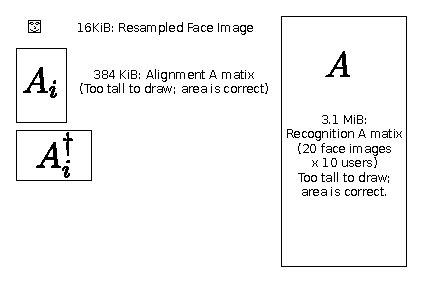
\includegraphics[scale=1.2]{figures/arrays}
	\label{fig:arrays}
}
\subfigure[The caches on a E5530 CPU]
{
	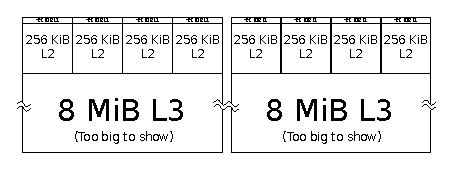
\includegraphics[scale=1.2]{figures/cpu_caches}
	\label{fig:cpu_caches}
}
\subfigure[The caches on a GTX480 GPU]
{
	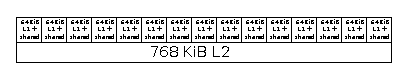
\includegraphics[scale=1.2]{figures/gpu_caches}
	\label{fig:gpu_caches}
}
\label{fig:caches}
\caption{A visual comparison of the algorithm working set to the CPU and GPU
caches.  Note: Although the aspect ratio could not be preserved, all arrays and
caches are drawn so that the area is proportional to the size of the data. }
\end{figure}

% CPU CACHE DISCUSSION
%2MB = 2**21 bytes
%64*64*4 = 2**14 bytes = 16384 bytes per image
%... so can fit 2**7  = 128 images.
Each core has a private 32\,KiB L1 data cache and a private 256\,KiB L2 cache.
%16MB = 2**24 bytes = 16777216 bytes
%64*64*4 = 2**14 bytes = 16384 bytes per image
%... so can fit 2**10  = 1024 images.
Each processor further has 8\,MiB of L3 cache that is shared by the four cores.
Overall, the algorithm has approximately 16\,MiB of L3 cache
available for a dual-processor configuration.  

For floating-point instructions, each core also has a vector processing unit
(SSE) capable of performing the same arithmetic operation on four single-precision 
floating point values simultaneously.
There are thus two important levels of concurrency that need to be exploited to
efficiently use a modern CPU: {\em core-level} concurrency and {\em sse-level}
concurrency. 

\subsection{GPU Hardware Concurrency}
The main defining characteristics of contemporary multi-core GPU architectures
are that they have two (much wider) levels of concurrency, relatively small amounts of
 cache, and relatively low clock speeds.  Whereas most of the transistors on
a typical CPU are dedicated either to cache or to hardware that enables higher
clock speeds (such as branch prediction, out-of-order instruction execution, etc...),
most of the transistors on a GPU are dedicated to arithmetic logic units.
An explanation of the CUDA programming model at a useful level of completeness would take 
more space than is available here, so we will instead frame our discussion in terms of 
hardware capabilities. \footnote{A discussion of the CUDA programming model can be found
in the NVIDIA C for CUDA Programming Guide}

Our target GPU architecture is the Nvidia Fermi architecture (\eg, the GTX 480
GPU used in this paper).  CUDA based GPUs are comprised of several
\emph{streaming multiprocessors} (SMP), each of which is roughly analogous to a CPU core.
For Fermi architecture GPU's, there are up to 16 SMP's, and each SMP is capable of executing up to 64 single precision 
floating point operations
concurrently. \footnote{In CUDA terms, the warp width is 32, and the floating pipeline can
issue up to two warps simultaneously}

% GPU CACHE DISCUSSION
% for L2 cache
% 768KB = 786432 bytes
% 64*64*4 = 2**14 bytes = 16384 bytes per image
% 48 images
Each SMP contains its own L1-cache, which is divided between hardware managed
and software managed ("shared") memory.  Additionally, all SMPs share a common
L2-cache.  For our system, each SMP has 64 KiB of L1 cache, and all SMP's share
768KB of L2 cache. 
%The cache hierarchy 
The relatively small amount
of cache (1/23 as much as CPU L3) on the GPU is balanced by a significantly
higher bandwidth between the processor chip and off-chip memory (DRAM) compared
to the CPU.  A scale drawing of the caches available on the GPU can be seen in Figure \ref{fig:gpu_caches}.
The GPU has its own memory system, and any data the GPU uses must first be
transferred from CPU DRAM to GPU DRAM over PCI-Express.  For our application,
this transfer overhead can be amortized over a large amount of computation and is
not a major concern.

While the programming model for
the SIMD units of each SMP is somewhat more flexible than on the CPU,
leveraging the flexibility typically comes at the cost of reduced concurrency
.\footnote{In CUDA terms, code branches that cause warp divergence usually
result in serialization of the different groups of threads}  Therefore, for
the purposes of comparing hardware architectures, the SIMD units on the GPU are
roughly analogous to the CPU SIMD units. Thus, in summary, the GPU hardware 
provides two levels of concurrency: {\em SMP-level}
concurrency and {\em thread-level} concurrency.  Note that the GPU provides more
concurrency than a CPU at both levels (14 SMP's vs. 8 cores) and (64 wide vs. 4 wide SIMD
units).

\section{Parallelism in the Face Alignment Stage}
\label{sec:alignment}

Given the hardware concurrency in modern parallel computing architectures,
next, we shall study the optimal mappings of the algorithm parallelism in face
recognition to the multi-core CPUs and GPUs, respectively.  In this section, we
first focus on the face alignment stage (see Figure \ref{fig:pipeline}).

Face alignment \eqref{eq:l1min_alignment} estimates an image transformation
$\tau$ that rectifies the query image $\tilde{\bb}$ with possible pose
variation w.r.t. each training class $A_i$, which leads to the minimal sparsity
in error $\ee$ after the alignment. Note that directly solving
\eqref{eq:l1min_alignment} would require simultaneously estimating $\xx$,
$\ee$, and $\tau$ typically on a nonlinear manifold, which renders the problem
extremely difficult to solve exactly with many local minima.

To mitigate the problem, if the system can obtain a good initial guess of the
transformation $\tau$ (\eg, provided by a good face detector), the optimal
solution for $\tau$ can be sought iteratively by linearization at each $j$th
step as follows:
\begin{equation}
\min_{\xx, \ee, \Delta \tau_j}\|\ee\|_1\quad \subj\quad \tilde\bb\circ\tau_j +  J_j\Delta \tau_j = A_i\xx + \ee,
\end{equation}
where $J_j = \nabla_{\tau_j}(\tilde\bb\circ\tau_j)$ is the Jacobian, and
$\Delta \tau$ is a step update to $\tau$. Denote $\bb_j =
\tilde\bb\circ\tau_j$, $B_j = [A_i, -J_j]$ and $\ww^T = [\xx^T, \Delta
\tau^T]$, then the update $\Delta \tau$ can be computed by solving the
following linear program:
\begin{equation}
\min_{\ww, \ee}\|\ee\|_1\quad \subj\quad \bb_j = B_j\ww + \ee.
\label{eq:alignment-linearization}
\end{equation}
%If the warping $\tau$ is constrained to be a similarity transform,
%it can be paramaterized in such a way that the computation of $\frac{\partial \bb}{\partial \tau_p}$
%reduces to several linear vector operations involving pixel coordinates $(u,v)$, $\tau \in \Re^4$,
%and the image gradients $\f_x, \f_y \in \Re^M$, the latter of which only has to be computed
%once per test image.  
The per-class alignment algorithm via ALM is summarized in Algorithm
\ref{alg:iterative_alignment}. 
%In terms of computational complexity, one significant
%term is the computation of the matrix pseudo-inverse $B_j^\dagger$, whose
%computational cost is bounded by $O(n_i^2m + n_i^3)$. However, for per-class face
%alignment, since both $B_j$ and $J_{j}$ are very tall matrices (\ie, $m\gg n_i$
%for all $i=1, \cdots, K$ classes), we find that the computation cost is still
%dominated by the frequently computed matrix-vector multiplications in the
%inner loop.
\begin{algorithm}[ht!]
\caption{\bf (Face Alignment via ALM)} \label{alg:iterative_alignment}
{\bf Input:} $\bb$, $A_i$, $\x_0 = \mathbf{0}$, $\tau_0$, and $J_0$.
\begin{algorithmic}[1]
\WHILE{not converged ($j = 1,2,\ldots$)}
\STATE Update $\bb_j \leftarrow \frac{\bb\circ \tau_{j-1}}{\|\bb\circ \tau_{j-1}\|}$; $B_j= [A_i, -J_{j-1}]$ and corresponding $(B_j^\dagger)^T$
\STATE Initialize $\ww_0 = \mathbf 0$, $\yy_0 = \mathbf 0$
\WHILE{not converged ($k = 1,2,\ldots$)}
\STATE $\uu_0\leftarrow \ww_{k-1}$; $\zz_0\leftarrow \ee_{k-1}$
\WHILE{not converged ($l = 1,2,\ldots$)}
\STATE $\zz_l \leftarrow \mbox{shrink}\left(\bb_j - B_j\uu_{l-1} + \frac{\yy_{k}}{\mu_{k-1}}, \frac{1}{\mu_{k-1}}\right)$
\STATE $\uu_l \leftarrow B_j^\dagger \left(\bb_j - \zz_{l} + \frac{\yy_{k-1}}{\mu_{k-1}} \right) $
\ENDWHILE
\STATE $\ww_k \leftarrow \uu_l$; $\ee_k \leftarrow \zz_l$
\STATE $\yy_{k} \leftarrow \yy_{k-1} + \mu_{k-1} (\bb_j - B_j\ww_{k} - \e_{k})$
\STATE $\mu_{k} \leftarrow \rho\mu_{k-1}$
\ENDWHILE
\STATE Update $\ee_j$, $\tau_j$, and $J_j$
\ENDWHILE
\end{algorithmic}
{\bf Output:} $\tau_i^*\leftarrow \tau_j, \e_i^*\leftarrow \ee_j$
\end{algorithm}

In summary, the alignment stage essentially contains two levels of available
parallelism. At the higher level, there are per-class alignment problems
that are solved independently, or \emph{problem-level parallelism}.  At a lower
level, the first-order linear algebraic operations exhibit parallelism within
image operations, \ie, at the pixel level.  We call this \emph{pixel-level
parallelism}.  In the following two sections will will discuss how to
exploit these two levels of parallelism on different CPU and GPU architectures.

\subsection{CPU Implementation} 
\label{sec:alignment_implementation_cpu}

Optimal implementation of Algorithm \ref{alg:iterative_alignment} on a multi-core CPU must take 
into account the properties of the cache hierarchy. In general, cache that is 
closer to the core (i.e. L1 cache) has higher bandwidth, but smaller size compared to cache
that is farther from the core (L3 cache).  For reference, Figure \ref{fig:cpu_caches} 
shows the the sizes of L2 and L3 caches of the Intel E5530 CPU, 
which is a representative example of a modern multi-core CPU. 

For the E5530, the L2 cache in each core is only able to store about 16 images.
For image alignment problem, the number of training images per class is
typically larger than 16.  Therefore, if eight instances of
\eqref{eq:alignment-linearization} were be executed in parallel on the eight
cores, there would be an insufficient amount of L1 or L2 cache to hold $B_j$ and
$B_j^\dagger$ during the iterative process to execute Algorithm
\ref{alg:iterative_alignment}. Therefore, the bottleneck in this strategy becomes the
bandwidth between the L2 cache and L3 cache. The implementation of some
previous works \cite{WagnerA2009-CVPR,WagnerA2011-PAMI} is indeed based on this
mapping strategy.

In this paper, we show that for CPU parallelism of face alignment, a higher
performance implementation can be achieved by {\em not} taking advantage of
problem-level parallelism at all, and instead mapping the pixel-level parallelism
onto both the core-level and the SSE-level concurrency provided by the CPU.  In
other words, the proposed CPU implementation performs alignment of a query
image against the training images of a single user at a time using all cores on
both processors.

More specifically, in our implementation, most of the operations take
advantage of Intel Math Kernel Library (MKL), a commercial implementation of
the standard Basic Linear Algebra Subprograms (BLAS). For the image resampling
step, we make use of the Intel Integrated Performance Primitives (IPP) library.
Both MKL and IPP are optimized for Intel multi-core CPUs, and are able to
automatically utilize both core-level and vector-level concurrency. For other
operations that are not optimized by Intel in-house libraries, such as the shrinkage
operator in step 7 of Algorithm \ref{alg:iterative_alignment}, we achieve both
vector-level and core-level concurrency through a combination of the Open MP
API \cite{dagum2002openmp} and the automatic vectorization facilities of the
Intel C++ compiler (ICC) \cite{dulong1999overview}. 
%We shall compare the performance of the two parallelism methods in Section \ref{sec:experiment}.

\subsection{GPU Implementation}
\label{sec:alignment_implementation_gpu}
While on the CPU, algorithm performance is highly dependent on effective
cache usage, on the GPU cache is relatively unimportant for ALM based
$\ell_1$-min.  As can be seen in Figure \ref{fig:caches}, the GPU has 
a very small amount of cache compared to the CPU.  While it might be possible
to fit a single instance of the alignment problem (with a slightly reduced problem size)
into L2 cache, this would not be an efficient use of the GPU's resources.
The strength of the GPU's memory architecture for our purposes it's ability to sustain a very
high bandwidth to DRAM.  A higher overall bandwidth can be achieved if 
many memory transactions are performed simultaneously, than can be achieved
with a large number of smaller transactions that are just large enough to fill
the L2 cache.

Therefore, whereas on the CPU we advocate performing alignment for one training
class at a time, on the GPU we advocate performing alignment for many classes
concurrently.  \footnote{In CUDA terminology, Our proposed alignment stage
implementation consists of a single kernel that performs alignment for all
subject classes.  Each instance of the alignment problem is assigned its own
thread block, and the GPU hardware schedules as many thread blocks to run
concurrently as the hardware will allow.} The number of subject classes that
actually get aligned concurrently is chosen by the GPU hardware. In our
experiments the hardware is able to schedule 4-5 classes per SMP to run
concurrently. This mapping of the problem-level parallelism onto the SMP-level
concurrency is illustrated in Figure \ref{fig:alignment_mapping_gpu}.

\begin{figure}
\centering

\includegraphics[width=3.4in]{figures/alignment_mapping_gpu}
\caption{Proposed mapping of alignment parallelism onto GPU concurrency}
\label{fig:alignment_mapping_gpu}
\end{figure}

The full resolution query image, along with its numerical derivatives in both
image directions, are stored in GPU texture memory. This  allows the
computation of $b(\tau)$ and $J(\tau)$, which essentially consist of warped
versions of the test image and its derivatives, to exploit the GPU's special
purpose hardware for bilinear interpolation.

Solving one alignment problem per SMP necessitated the implementation of a
custom CUDA routine for computing $B_j^\dagger = (B_j^TB_j)^{-1} B^T = G^{-1} B_j^T$. $G$
is inverted using Gaussian elimination with partial pivoting.  To achieve
precision comparable to the single precision LAPACK routines in Intel's MKL
with this simplistic algorithm, we use double precision.  Since $G$ is only $n
\times n$ and $B_j^\dagger$ is only computed once per optimization problem, the
cost of the inversion is dwarfed by the cost of other steps.  
Additionally, reductions on long vectors (i.e. sum or $\ell_1$ norm
of an image) are performed using a double precision temporary variable for accumulation.
%In Section \ref{sec:experiment}, we show the performance of our CPU and GPU
%implementations running on synthetic and real image data.

\section{Parallelization of the Face Recognition Stage}
\label{sec:recognition}
After the face alignment stage is complete, all but the 20 users with lowest
$||\e_i||_1$ are thrown out, $\bb$ and $A_i$ are re-sampled to a common alignment
using $\tau_i$, and $A_i$ are concatenated into a new matrix $A$.
A sparse representation of $\bb$ w.r.t $A$ is then recovered
by solving a single $\ell_1$-min problem, as shown
in \eqref{eq:l1min_denoise}, using Algorithm \ref{alg:alm_rec}.  The
coefficients $\x$ are then used to compute error residuals that are used for
classification.  
%This recognition algorithm has
%been extensively studied in
%\cite{WrightJ2009-PAMI,YangA2010-ICIP,WagnerA2011-PAMI}.
In this stage of the algorithm, there is no problem-level
parallelism to exploit, so this section will discuss how to exploit pixel-level parallelism
on both CPU and GPU hardware.
Then in Section \ref{sec:experiment}, we will benchmark the
performance of the two architectures and further demonstrate the speed
gains achieved by our proposed implementations over previously published implementations.

\begin{algorithm}[t]
\caption{\bf (Face Recognition via ALM)} \label{alg:alm_rec} 
\begin{algorithmic}[1]
\begin{small}
\STATE {\bf Input:} $\bb \in \Re^m$, $A \in \Re^{m \times n}$,
$\x_1 = \mathbf{0}$, $\e_1 = \bb$, $\y_1 =
\mathbf{0}$.
\WHILE{not converged ($k = 1,2,\ldots$)}
\STATE $\e_{k+1} = \textup{shrink}(\bb - A\x_k +
\frac{1}{\mu}\y_k, \frac{1}{\mu})$;
\STATE $t_1\leftarrow 1$, $\z_1 \leftarrow \x_k$, $\w_1 \leftarrow \x_k$;
\WHILE{not converged ($l = 1,2,\ldots$)}
\STATE $\w_{l+1} \leftarrow \textup{shrink}(\z_l +
\frac{1}{\gamma}A^T(\bb - A\z_l - \e_{k+1} +
\frac{1}{\mu}\y_k), \frac{1}{\mu\gamma})$;
\STATE $t_{l+1} \leftarrow \frac{1}{2}( 1 +
\sqrt{1+4t_l^2})$;
\STATE $\z_{l+1} \leftarrow \w_{l+1} + \frac{t_l - 1}{t_{l+1}}(\w_{l+1} - \w_l)$;
\ENDWHILE
\STATE $\x_{k+1} \leftarrow \w_{l}$,  \; $\y_{k+1} \leftarrow \y_k + \mu (\bb - A\x_{k+1} - \e_{k+1})$;
\ENDWHILE \STATE
{\bf Output:} $\x^* \leftarrow \x_k, \e^* \leftarrow \e_k$.
\end{small}
\end{algorithmic}
\end{algorithm}

\subsection{Recognition Stage Implementation} Compared to problem-level
parallelism, pixel-level parallelism in Algorithm \ref{alg:alm_rec} is
relatively easy to exploit using existing BLAS libraries.  For this reason,
both the CPU and GPU implementation of the recognition stage is very similar to
the CPU implementation of the $\ell_1$-min advocated in Section
\ref{sec:alignment_implementation_cpu}.  On the CPU, most of the operations map
well onto MKL BLAS calls, and the operations that do not can be easily
parallelized using OpenMP and auto-vectorization.

On the GPU, most of the operations map well onto similar calls in Nvidia's GPU
BLAS library (CUBLAS) which, like MKL, can take advantage of both levels of
concurrency available in the hardware architecture.  Operations that do not map
well onto the CUBLAS API were implemented as GPU kernels (in C for CUDA).
Additionally, some operations that could have been implemented via multiple
BLAS calls, performance improvements were achieved by combining multiple
vector-vector operations into a single kernel, due to reduced bandwidth and
kernel call overhead.  

In order to avoid expensive data transfer across the bus connecting the GPU
card and the CPU motherboard (the PCI express bus), all of the data is
transferred to GPU DRAM once, and all non-trivial tasks are performed on the
GPU on data stored in GPU DRAM.  
All non-scalar temporary variables are stored in GPU DRAM
during solver execution. 
%with the sole exception of the pseudo-inverse of $B_j$,
%which is computed on the CPU via Intel's LAPACK implementation, and then
%uploaded to GPU DRAM.  

\section{Experiments} \label{sec:experiment} In this section, we benchmark the
performance of our parallel implementations of $\ell_1$-min on CPU and GPU
platforms.  In order to show how our $\ell_1$-min algorithms scale with problem
size, in Section \ref{sec:simulation} we will begin with benchmarks for the
general $\ell_1$-min problem on synthetic data.  We will then progress in
Section \ref{sec:benchmark} to demonstrating the speed and accuracy of our
implementations as applied to the alignment and recognition stages of the face
recognition problem.

To generate a meaningful comparison between different hardware architectures,
in all cases we compare the performance of hardware architectures on a
per-board basis:  For CPU implementations, the benchmark makes use of all of
the cores in as many CPU's are present.  For GPU implementations, the benchmark
makes the best use of the entire GPU chip (most GPU boards have a single GPU
chip).  Aside from the exceptions already mentioned in Section
\ref{sec:alignment_implementation_gpu}, all math operations are performed in
single precision.

\subsection{Simulations on Random Data}
\label{sec:simulation}

The first experiment compares the performance of our two proposed
implementations of the general $\ell_1$-min (Algorithm \eqref{alg:alm}) given a
generic random matrix $A$ and a random sparse vector $\xx_0$.  The measurement
$d \times n$ matrix $A$ is generated as a random Gaussian matrix, with each
entry randomly generated from the standard normal and normalized with unit
column norm.  The ratio of $d/n$ is fixed at $1/2$ with $n$ varying from 1000 to 8000.
The ground truth signals, $\xx_0$ have a sparsity rate of 10\% of d with
elements sampled from a normal distribution and normalized to unit $\ell_2$ vector
norm.  Because the ground truth signal $\xx_0$ is known, the algorithm
terminats when $\|\bx-\bx_0\| < \tau$ with $\tau=10^{-3}$.  The measurement
vector is generated with the equation $\bb_0 = A \xx_0$.   

The results of this benchmark can be found in Figure \ref{fig:random_data}.
The x-axis represents the size of the $A$ matrix and the y-axis represents the
average amount of time it to complete a single problem instance.  The GPU
implementation tends to be faster than the CPU implementation at solving a
single large problem, whereas the CPU implementation is faster at solving a
single small problem.  
\begin{figure}
\begin{center}
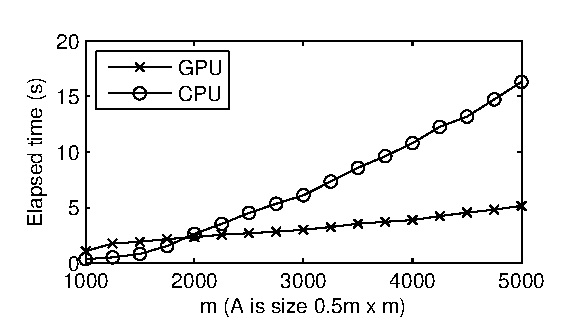
\includegraphics[width=3.5in]{figures/time_vs_matrix_size_constant_tol}
\end{center}
\caption{Comparison of $\ell_1$-min runtime vs. dimensions of $A$ on random data.}
\label{fig:random_data}
\end{figure}

\subsection{Face Recognition Pipeline Benchmark} 
\label{sec:benchmark}
This section presents benchmarks of our CPU and GPU implementations of the
alignment stage of the face recognition pipeline, as shown in Algorithm
\ref{alg:iterative_alignment}, as well as the recognition stage of the
face recognition pipeline, as seen in Algorithm \ref{alg:alm_rec}.

First, in order to test our theory that the GPU performs best solving many
$\ell_1$ problems-per concurrently, we benchmark three implementations of the
alignment $\ell_1$-min solver with $A$ of size $5120 \times 32$, and a fixed
$50$ inner loop iterations for each of $50$ outer loop iterations. The runtime
on a GTX480 GPU is averaged over a large number of trials, which are run
sequentially or concurrently depending on the implementation.
The results are shown in Table \ref{tbl:ubench}.
Our proposed parallelization of the $\ell_1$-min used in the alignment
stage is {\em eight times} faster than an implementation solving a single
problem at a time using the stock BLAS libraries.
\footnote{Note that the streams implementation is limited significantly by a 
cap on the number of concurrent streams in the current version of CUDA}
%The results are shown below:
\begin{table}[h!]
\caption{Benchmark of implementations of alignment $\ell_1$-min.}
\begin{tabular}{|l|c|}
\hline
Sequential solver using CUBLAS & 302\,ms \\
\hline
One problem per SMP using CUDA streams & 70\,ms  \\
\hline
Four problems per SMP using single kernel & {\bf 36\,ms} \\
\hline
\end{tabular}
\label{tbl:ubench}
\end{table}
 
Using an implementation motivated by the previous result, we now benchmark our
iterative alignment implementation on real face data.  For experiments on face
data we use subsets of the CMU Multi-PIE Face Database.  For gallery images we
use frontal images from session 1, which contains 20 images per user taken
under different illuminations. For test images we use images from session 2.
The training images are prepared as follows: The iterative alignment stage
seeks a similarity transformation between the coordinate frame of the "camera"
resolution test image and the coordinate frame of the "canonical" resolution
images which the images are compared.  We use a $64 \times 64$ pixel window in
the canonical frame.  The training images are aligned by manually clicking the
two outer eye corners in the camera frame, and then warping the images via a
similarity transformation such that the eye corners lie at a pair of canonical
eye locations in the canonical frame.  The canonical eye corners are chosen
such that for well aligned images, the canonical window contains exclusively
pixels from the subject's face.  We assume the face detector is accurate, so
for the test images we use clicked eye corners for test image alignment
initialization.\footnote{Previous publications have shown that iterative
alignment improves recognition accuracy substantially even with clicked eye
corners}

Figure \ref{fig:alignment_stage_runtime} shows the average run time of the CPU and GPU implementations to align
a query image against all the subject classes separately. We vary the number of
subject classes to show how the algorithms scale. 
\begin{figure}
\centering
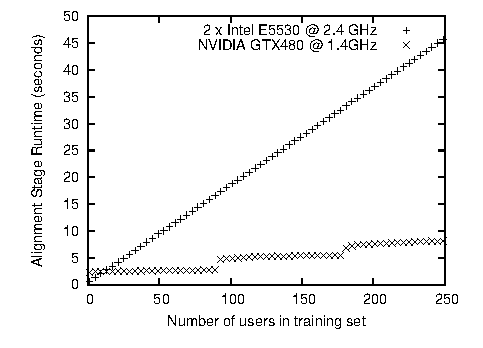
\includegraphics[width=3.4in]{figures/alignment_runtime_graph}
\caption{Alignment stage runtime vs. size of training database.}
\label{fig:alignment_stage_runtime}
\end{figure}
Similar to the results in Figure \ref{fig:random_data},
there is a crossover point above which the GPU out-performs the CPU.  Since
the CPU algorithm solves problems sequentially, there is a linear trend.  
The tiers seen in the GPU profile result from the GPU hardware scheduling alignment
problems in concurrent batches, but the overall trend is linear as expected.

%The following experiment fulfills the dual purpose of verifying the accuracy of
%the alignment stage, and motivating a threshold on how many users are kept for
%the recognition stage.  Setting this threshold establishes a compromise between
%recognition speed and potential recognition rate.  To explore the affect of the
%threshold on potential recognition rate, we vary the number of users kept for
%the recognition stage and estimate the probability of the test user being
%among the set of training users kept for the recognition stage.  This curve
%bounds above the achievable recognition rate of the overall pipeline.  As can
%be seen in Figure \ref{fig:user_alignment_rank_plot}, there are rapidly
%diminishing returns as the number of kept users is increased beyond 20; a small
%fraction of the gallery.
%\begin{figure} 
%\centering
%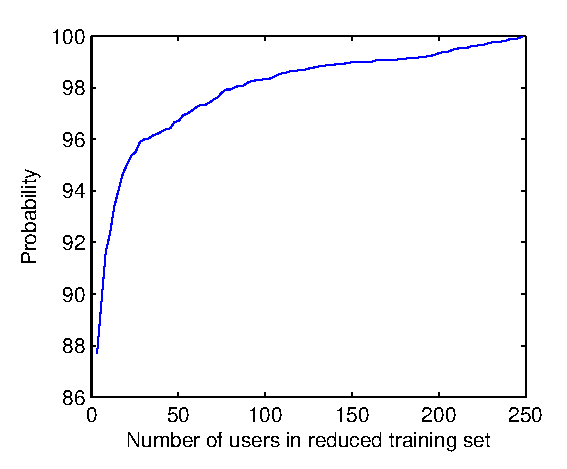
\includegraphics[width=3.4in]{figures/user_alignment_rank_plot}
%\caption{Probability of the test user being kept for the recognition stage vs.
%number of training users kept for the recognition stage.}
%\label{fig:user_alignment_rank_plot} \end{figure}

\begin{figure} 
\centering
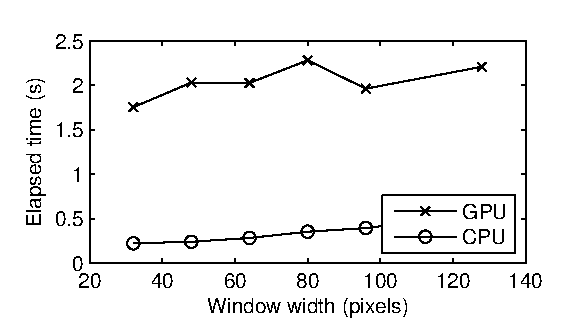
\includegraphics[width=3.4in]{figures/speedVsResolution}
\caption{Recognition stage runtime vs. size of training database.}
\label{fig:recognition_stage_runtime} \end{figure}

Finally, we perform an experiment verifying the recognition accuracy of the
overall pipeline.  Since one would expect higher recognition rates but longer
execution time for higher resolution images, we compare the recognition rate of
the overall pipeline with the face recognition stage run at 5 different
canonical image resolutions: $32\times32, 48 \times 48, 64 \times 64, 96 \times
96, \textrm{and} 128 \times 128$.  As motivated by Figure
\ref{fig:user_alignment_rank_plot}, we fix the number of gallery users to 20,
giving approximately 95\% probability to have the true user in the training
set.  
%The inner loop tolerance to 1e-5 and outer loop tolerance to 1e-2.  
\begin{figure}
\centering
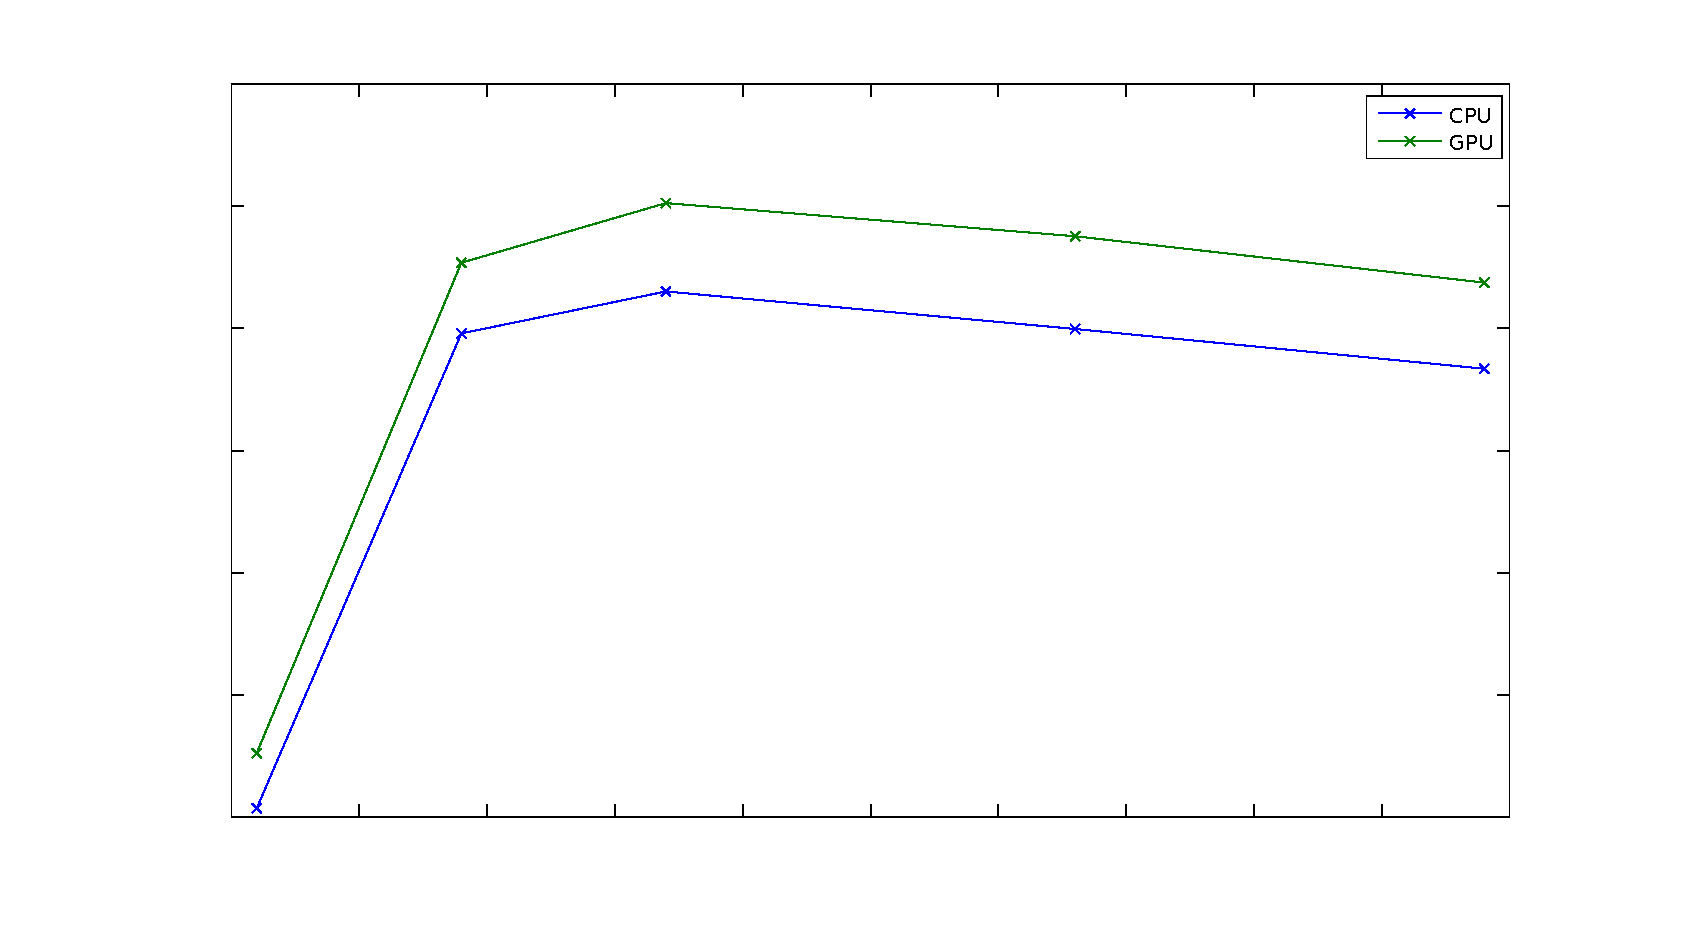
\includegraphics[width=3.4in]{figures/accuracyVsResolution}
\caption{Recognition rate of the full pipeline vs. face window resolution.}
\label{fig:accuracy_vs_resolution}
\end{figure}
As can be seen in Figure \ref{fig:accuracy_vs_resolution}, at the optimal
resolution, which happens to match the alignment stage resolution, this bound
is very nearly achieved by the GPU implementation.  For significantly lower
resolutions, the accuracy drops off significantly.  Of the two main stages of
the face recognition pipeline, the iterative alignment stage is by far the most
expensive; the recognition stage requires less than one second.

\section{Conclusion}
We have shown that our proposed parallelization is {\em eight times} faster
than an implementation solving a single problem at a time using the stock
CUBLAS library. Furthermore, the proposed mapping of the parallelism of the
face alignment problem onto the concurrency provided in modern CPU and GPU
architectures results in dramatic improvements in recognition speed over
previously reported implementations of the same pipeline.  Whereas earlier
implementations required over a second to align a test image against just one
of the 250 users in Multi-PIE session 1, the proposed CPU implementation can
perform the same task in only 45 seconds, and the GPU implementation can do it
in {\bf under 10 seconds}!.  In principle, the parallelization techniques
presented here make it feasible to implement an access control system for
hundreds of users on a handful of purpose-build multi-GPU workstations.

%We argue that in addition to vendor supplied libraries
%that attempt to leverage both levels of concurrency of the GPU, there is a need
%for standard libraries that operate at the SMP level of concurrency.

{\small
\bibliographystyle{ieee}
\bibliography{faces}
}

\end{document}

